% METODOLOGIA------------------------------------------------------------------

\chapter{METODOLOGIA}
\label{chap:metodologia}
Nessa seção, são descritas as etapas do desenvolvimento dessa monografia, sendo elas a formulação e pré-processamento da base de dados, a configuração da rede neural e sua codificação utilizando o \textit{framework} \textit{keras} \cite{chollet2015keras}, além de pesquisas e aplicações de melhorias para a rede neural proposta como o \textit{data augmentation} e a inicialização dos pesos a partir de valores de uma rede já treinada.

\section{Formulação da base}
No aprendizado de máquina, a base de dados em que foram feitos os treinos e os testes do método escolhido devem possuir um balanceamento na distribuição de amostras por classes, e as amostras de uma mesma classe devem possuir características que as diferenciem das outras amostras de outras classes.

\par Nesse trabalho foi feito a classificação de imagens de comida, dessa maneira a base montada contém imagens segregadas em classes como \textit{pizza} e \textit{sushi}. Também foram adicionadas classes de imagens que não estão relacionadas com comida, como \textit{plant}(no português, planta) e \textit{domestic animals}(no português, animais domésticos), visando melhorar o classificador, quando utilizado em bases que possuam imagens não associadas a comida.
\par As imagens utilizadas para a formulação da base de dados desse trabalho foram retiradas das bases de dados \textit{ImageNet}\cite{deng2009imagenet} e \textit{Food-101}\cite{bossard14}. A base \textit{ImageNet} é densamente estruturada e organizada em hierarquia de árvore, facilitando assim encontrar as categorias que estão relacionadas ao tema abordado. Já base \textit{Food-101} é composta de 101 classes de imagens de comida, selecionadas e com um tamanho fixo de 1000 imagens por classe. A precisão de categorização das bases \textit{ImageNet} e \textit{Food-101} são necessárias para a formulação da base de teste deste projeto, tendo em vista que a categorização manual de imagens não seria uma abordagem viável, uma vez que redes neurais convolucionais demandam uma grande quantidade de imagens para um treinamento adequado.  

\par A base formulada possui um total de 16000 imagens separadas em 16 classes, sendo dessas classes 13  relacionadas com comida (\textit{chocolate cake, french fries, hamburger, ice cream, pizza, spaghetti bolognese, sushi,club sandwich, filet mignon, fried rice, hot dog, steak, tacos}) e três não relacionadas com comida (\textit{domestic animal, people, plant}). A diversidade dessas imagens seguem como exemplo na \autoref{fig:imagebase}.
\begin{figure}[H]
  \centering
  \caption{Exemplos de imagens encontradas na base de dados.}
  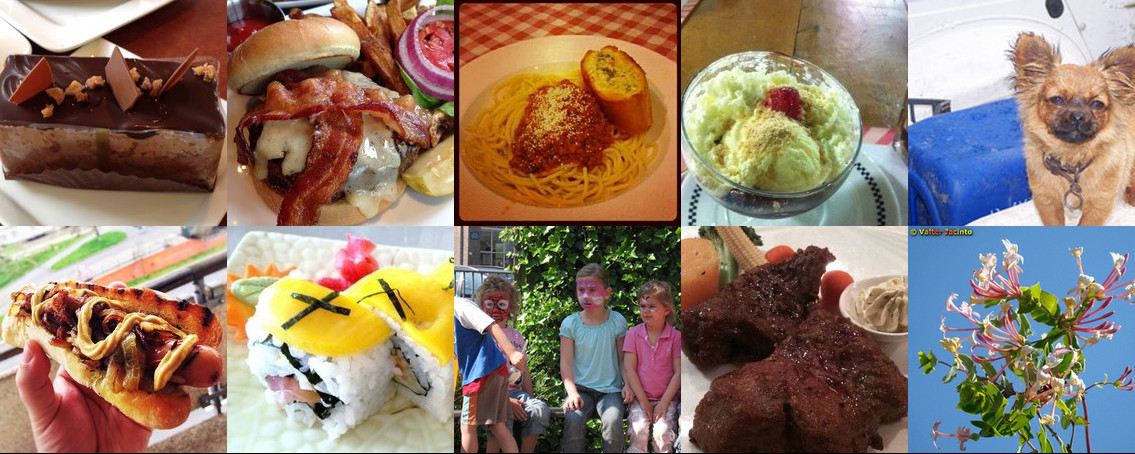
\includegraphics[width=300pt]{dados/figuras/imagembase}
  \fonte{imagens retiradas das bases \textit{ImageNet}\cite{deng2009imagenet} e \textit{Food-101}\cite{bossard14}}
  \label{fig:imagebase}
\end{figure}

\subsection{Pré-processamento}
\par Redes neurais convolucionais requerem de uma grande quantidade de imagens, dessa maneira as entradas fornecidas para a rede neural devem seguir um padrão, onde todas as imagens devem possuir as mesmas dimensões. Assim as imagens foram redimensionadas para 227x227 \textit{pixels}, tendo em vista que é um valor que obteve bons resultados em trabalhos semelhantes \cite{imaginetArticle}. Nas alterações de dimensões das imagens foi realizado um corte nas imagens originais para forçar uma formato quadrado antes de ser aplicado o redimensionamento, preservando os formatos das imagens.
\par Para a realização dos treinos e testes com a rede neural a base de dados foi separada em dados de treino e dados de teste. Como informado na \autoref{tab:base_images} 70\% das imagens (11200 imagens) de cada classe serão utilizadas para o treino da rede neural, e os 30\% das imagens restantes (4800 imagens) serão utilizadas para a fase de teste da rede neural.

\begin{table}[H]
    \centering
    \caption[Disposição da base de dados]{Separação da base de dados em classes, sendo informada a quantidade de amostras separadas para realizar as etapas de treino e teste, também é informado a base de origem do dado.
    \label{tab:base_images}}
    \begin{tabular}{ccccc}
        \toprule
             Classe & Amostras de treino & Amostras de teste & Amostras totais & Base de origem \\
        \midrule
            chocolate cake & 700 & 300 & 1000 & \textit{Food-101}\\
            french fries & 700 & 300 & 1000 & \textit{Food-101}\\
            hamburger & 700 & 300 & 1000 & \textit{Food-101}\\
            ice cream & 700 & 300 & 1000 & \textit{Food-101}\\
            pizza & 700 & 300 & 1000 & \textit{Food-101}\\
            spaghetti bolognese & 700 & 300 & 1000 & \textit{Food-101}\\
            sushi & 700 & 300 & 1000 & \textit{Food-101}\\
            club sandwich & 700 & 300 & 1000 & \textit{Food-101}\\
            filet mignon & 700 & 300 & 1000 & \textit{Food-101}\\
            fried rice & 700 & 300 & 1000 & \textit{Food-101}\\
            hot dog & 700 & 300 & 1000 & \textit{Food-101}\\
            steak & 700 & 300 & 1000 & \textit{Food-101}\\
            tacos & 700 & 300 & 1000 & \textit{Food-101}\\
            domestic animal & 700 & 300 & 1000 & \textit{ImageNet}\\
            people & 700 & 300 & 1000 & \textit{ImageNet}\\
            plant & 700 & 300 & 1000 & \textit{ImageNet}\\

        \bottomrule
    \end{tabular}
\end{table}



\section{Configuração da Rede Neural}

A configuração da rede neural convolucional utilizada nesse projeto é fundamentada na rede neural \textit{AlexNet} definida por \citeonline{imaginetArticle}. Essa rede utiliza de 8 camadas ocultas de processamento, sendo cinco camadas convolucionais e três camadas fortemente conectadas. Tendo em vista que a rede utilizada como exemplo foi estruturada para classificar mil classes, é necessário fazer algumas adaptações para classificar uma quantidade menor de classes, uma dessas alterações é a modificação da função \textit{softmax} para obter o resultado da classificação na última camada conforme descrito na \autoref{fig:arqrede}.

\par A primeira camada de convolução da rede separa a entrada, uma imagem de 227x227X3 em 96 núcleos de 11x11x3 (com uma distancia de 4 \textit{pixels} entre os centros das imagens vizinhas), onde cada imagem gerada é processada separadamente. Após essa camada é aplicada uma camada de \textit{max pooling}.

\par A segunda camada convolucional tem como entrada a saída da primeira camada convolucional normalizada e com \textit{pooling} aplicado, essa entrada é filtrada em 256 núcleos de 5x5x48. Após esse camada também é aplicado uma camada de \textit{max pooling}.

\par A terceira camada convolucional possui 384 núcleos de 3x3x256 que são conectados a entrada fornecida pela saída da segunda camada convolucional normalizada e aplicado o \textit{pooling}. As conexões entre a terceira, quarta e quinta camada convolucional, não possuem nenhuma operação de \textit{pooling} entre si. 
\par Assim a quarta camada convolucional possui 384 núcleos de 3x3x192 e a quinta camada possui 256 núcleos de 3x3x192. Após a quinta camada convolucional é aplicado uma camada de \textit{max pooling}.
\par A duas camadas seguintes são camadas fortemente conectadas com 4096 neurônios cada, com no fim de cada uma aplicada a função de \textit{dropout} inicialmente com uma taxa de 50\%. E por fim uma camada com 16 neurônios (um neurônio para cada classe) fortemente conectada com a operação de \textit{softmax} para obter a predição da entrada.

\begin{figure}[H]
  \centering
  \caption{Diagrama que representa a arquitetura da rede neural convoluciona proposta.}
  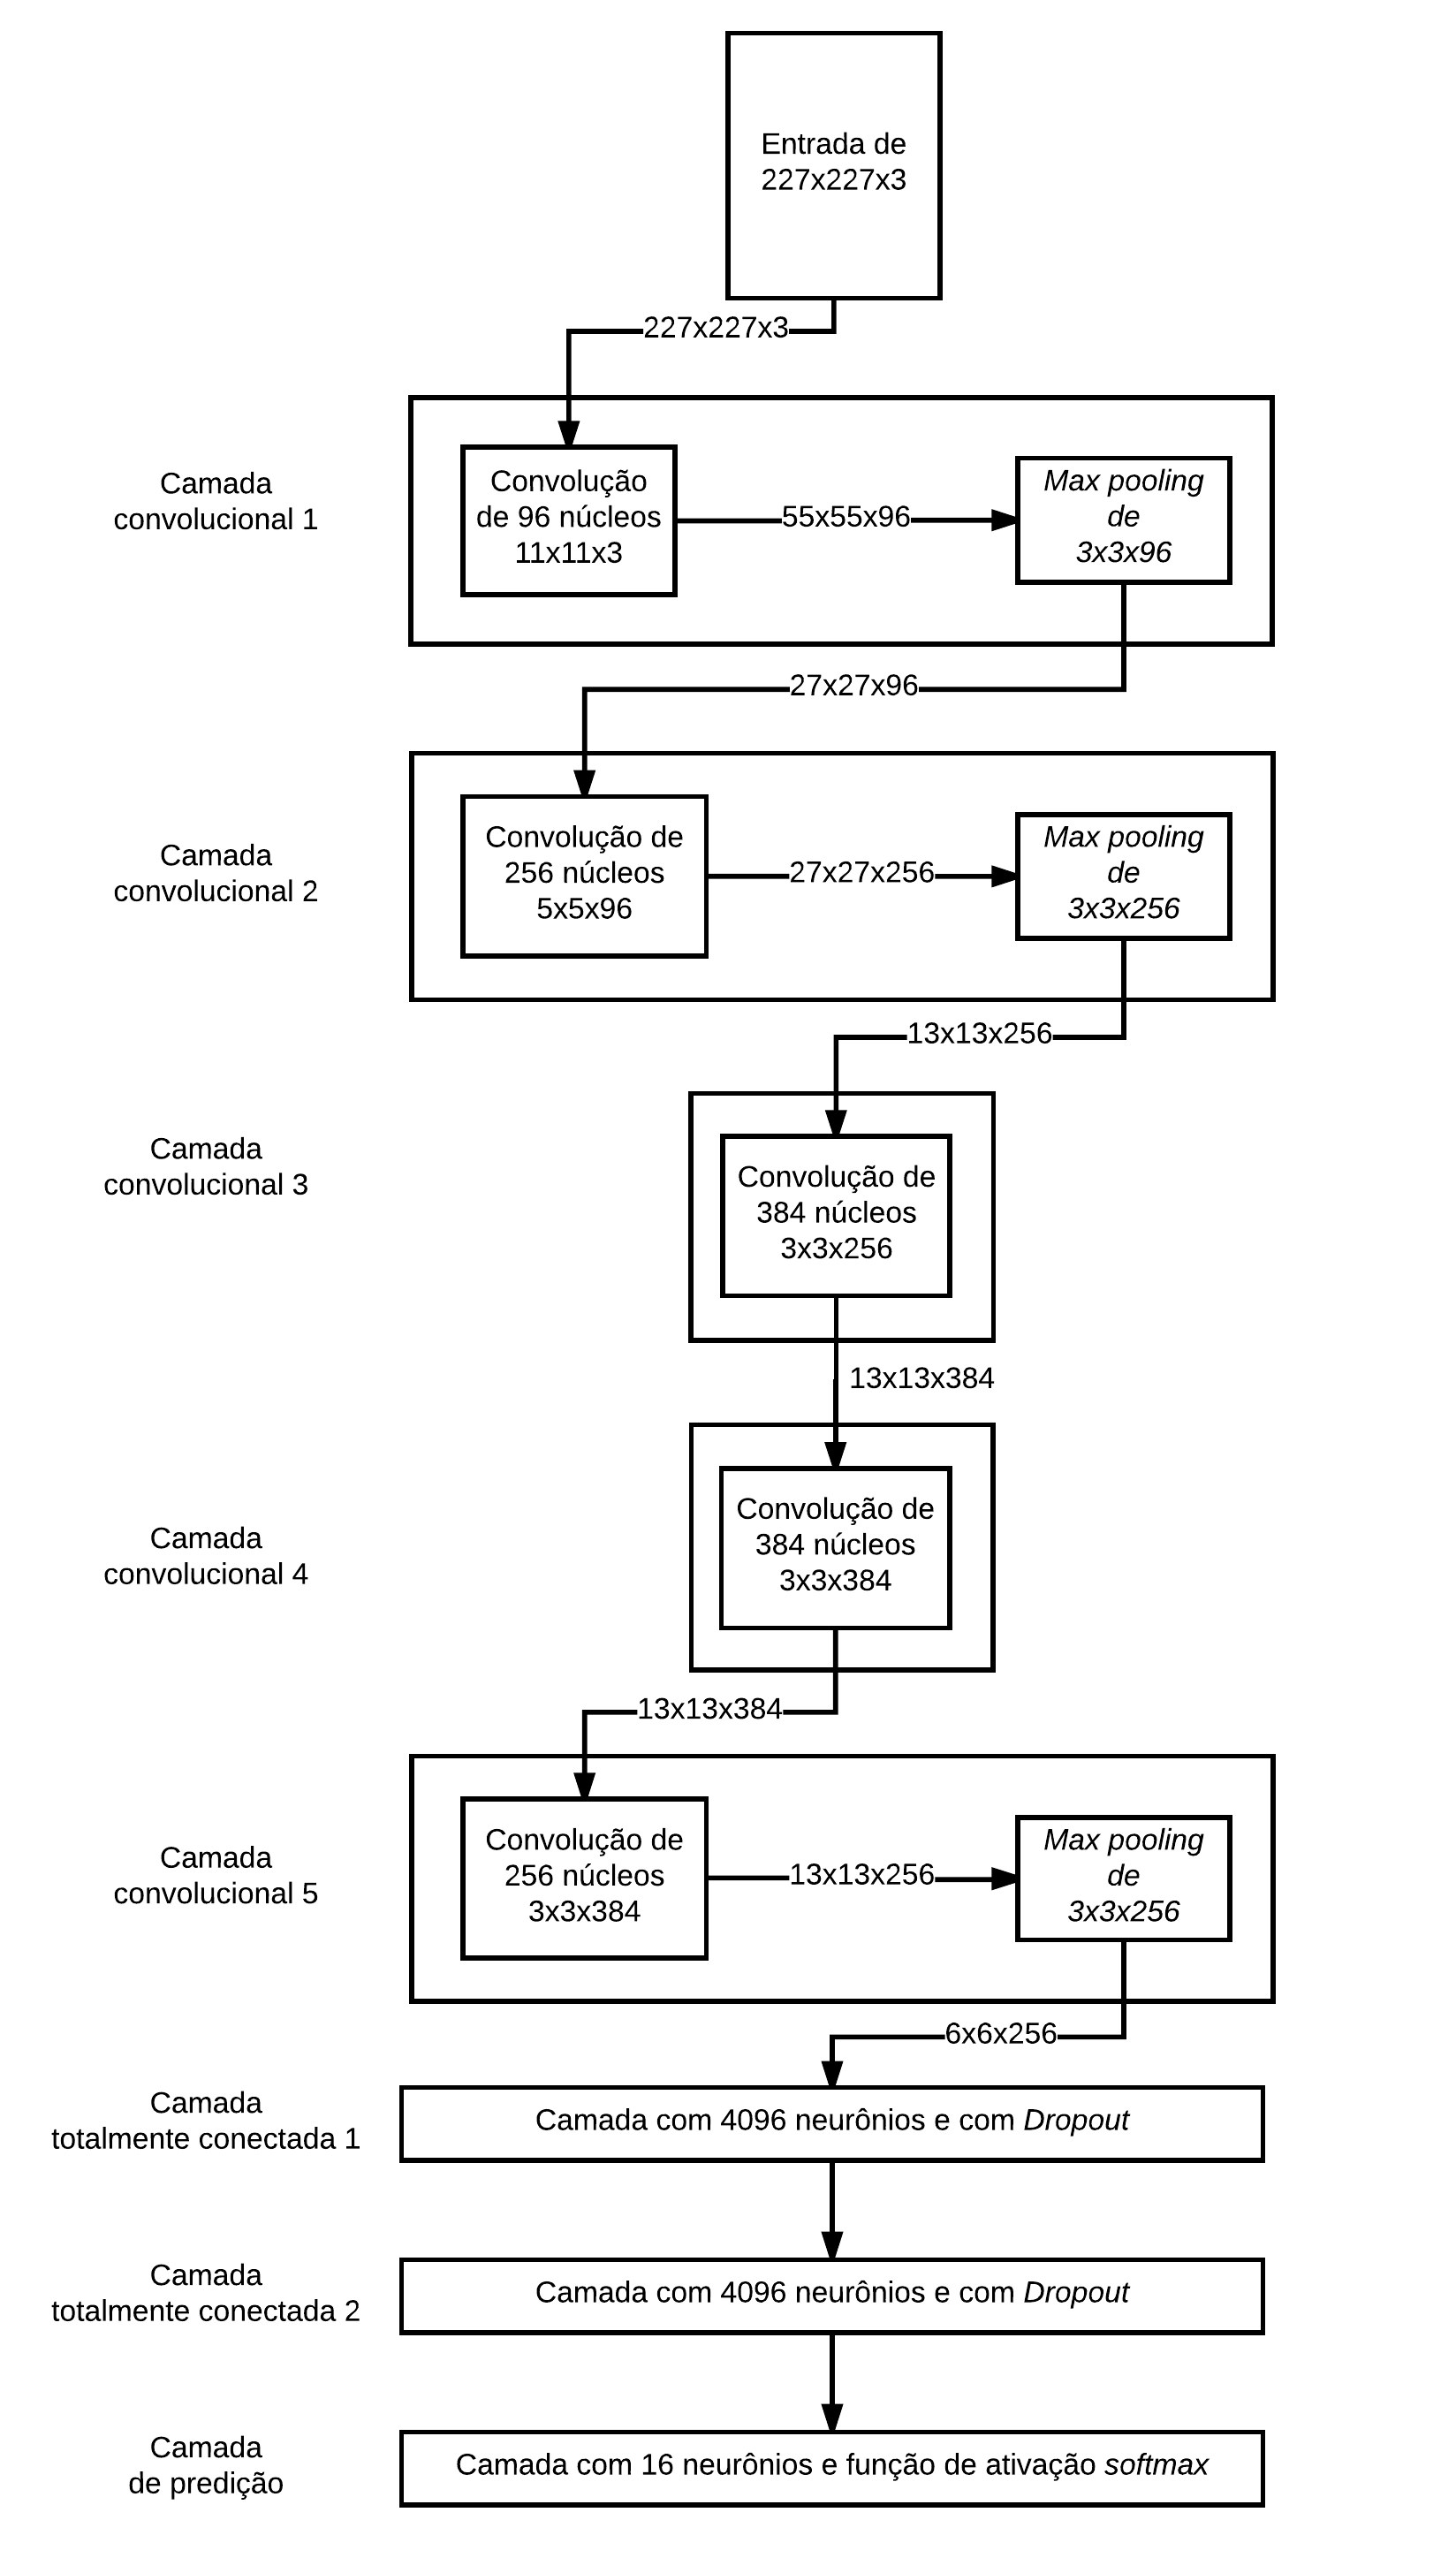
\includegraphics[width=500pt,angle=90]{dados/figuras/dia_rede}
  \label{fig:arqrede}
\end{figure}

\par Está sendo utilizado o \textit{framework} \textit{Keras} \cite{chollet2015keras} para descrever a rede neural. \textit{Keras} é um \textit{framework} em \textit{python} para execução de redes neurais utilizando \textit{GPU}(\textit{Graphics Processing Unit}). Com o \textit{keras} é possível configurar em alto nível uma rede neural, abstraindo a complexidade da descrição e implementação das rotinas de execução das camadas. Como exemplo de implementação temos a \autoref{fig:conv_keras}, contendo a codificação da primeira e segunda camada da rede neural proposta. Neste projeto o \textit{keras} está sendo utilizado com o \textit{back end Theano} \cite{2016arXiv160502688full} para a geração de código em \textit{Cuda}, linguagem que compila codigo para ser executado em GPU.
\begin{figure}[H]
  \centering
  \caption{Trecho de código com implementação utilizando o \textit{framework} \textit{keras} das duas primeiras camadas convolucionais da rede neural, contendo a definição da entrada e as implementações das camadas de transição entre as camadas de convolução um e dois.}
  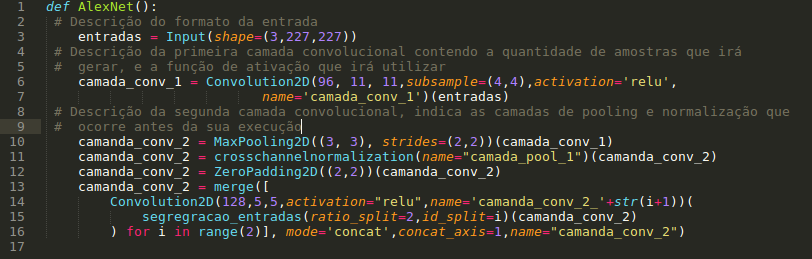
\includegraphics[width=400pt]{dados/figuras/exemplo_keras}
  \label{fig:conv_keras}
\end{figure}


\section{Melhorias para a rede neural proposta}

Melhorias no desempenho de redes neurais podem ser aplicadas em diversas etapas do processo de aprendizado e classificação. O aumento da base de treino, definir camadas serão para serem treinadas em determinadas épocas, a inicialização dos pesos da rede neural com valores de uma rede treinada com uma quantidade maior de amostras e o aprimoramento dos parâmetros de configuração da rede, são métodos que podem ser utilizados para aprimorar sua performance de classificação.

\par Nesse projeto foram aplicadas técnicas para a melhora na classificação, sendo elas
%técnicas o ajuste empírico da taxa de descarte de neurônios nas camadas totalmente conectadas,
o aumento dos dados na base de treino e a inicialização dos pesos da rede neural com pesos de uma rede já treinada. %Essas técnicas são descritas mais detalhadamente nas seções a seguir.

\subsection{\textit{Data augmentation}}
Uma técnica que vem sendo muito utilizada no para a redução do \textit{overfitting} na fase de treino de uma rede neural é a \textit{data augmentation} \cite{cui2015data}. 
Os dados da base são ligeiramente modificados, para obter aumento na quantidade de amostras.
Essas mudanças nas imagens podem ser inversões nos eixos, pequenas rotações, aproximações em certas partes das imagens ou até a aplicação da imagem em escala cinza.
Essa técnica tem o propósito de aumentar a quantidade de amostras em que serão realizados os treinos, buscando evitar um \textit{overfitting} \cite{imaginetArticle}.
\par Nesse projeto foi utilizada a técnica de \textit{data augmentation} aplicando inversão da imagem no eixo $y$, realizando um zoom de aproximação ou distanciamento de até 20\% da imagem e aplicado uma taxa de inclinação de até 0,2 radianos. As imagens são geradas com a combinação das transformações possíveis informadas, criando nove imagens para cada imagem de treino como representado na \autoref{fig:data_augmentation}. Essas imagens são geradas durante a execução do treino da rede e são armazenadas em memória.

\begin{figure}[H]
  \centering
  \caption{Imagem representado a técnica de \textit{data augmentation} aplicada na base de treino. A imagem no centro é a original, e as outras possíveis modificações aplicadas na imagem original, como a inversão do eixo $y$ e o aumento e diminuição do \textit{zoom}.}
  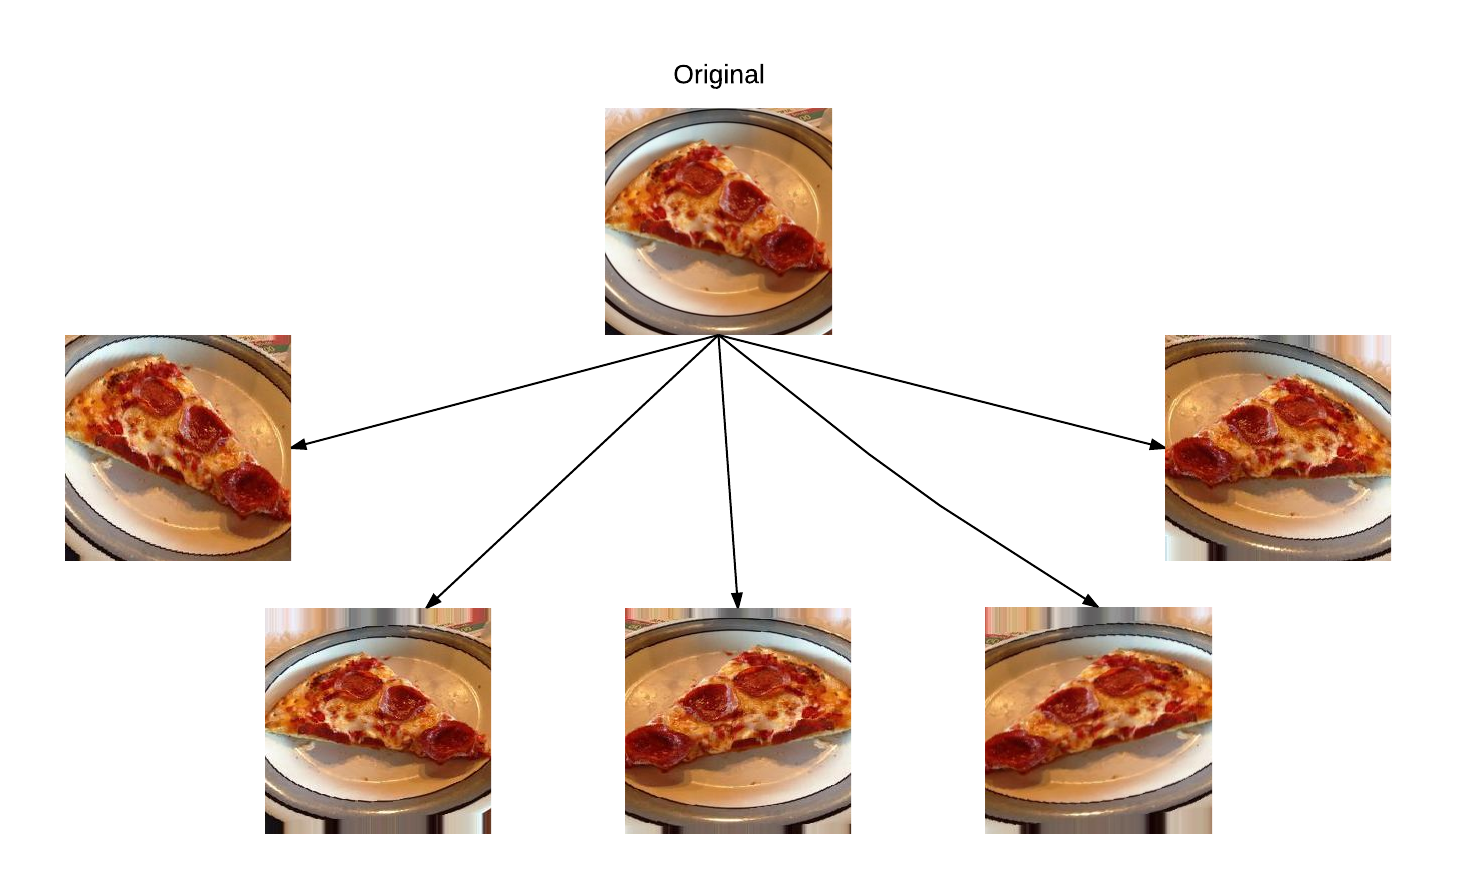
\includegraphics[width=400pt]{dados/figuras/data_augmentation}
  \fonte{Imagem produzida pelo autor (2017).}
  \label{fig:data_augmentation}
\end{figure}

\subsection{Inicialização dos pesos}
Uma rede neural treinado do inicio ao fim, tem seus pesos inicializados de maneira aleatória e conforme vai realizando suas predições os pesos são corrigidos para melhorar o poder de classificação. A inicialização dos pesos da rede neural com valores obtidos a partir de uma rede treinada, vem sendo utilizado como maneira de melhorar a classificação \cite{Girshick_2014_CVPR}. Geralmente os pesos vem de redes que treinaram uma quantidade muito grande de dados, conseguindo de certa forma transferir o aprendizado obtido para a rede que está inicializando os pesos. Nesse projeto foi realizado a inicialização dos pesos da rede neural, utilizando os pesos obtidos no treinamento da rede desenvolvida por \citeonline{imaginetArticle}.

% \subsection{Congelamento de camadas}

% \par O aprimoramento da rede neural convolucional pode ser feito por meio da utilização de parâmetros já treinados da rede neural, \cite{Girshick_2014_CVPR} descreve esse método como um pré-treino da rede, a preparando para a sua real tarefa. Podendo assim utilizar os pesos treinados em \cite{imaginetArticle} para um aperfeiçoamento da rede.
% \par Outro método utilizado para a melhora do resultado e redução do \textit{overfit}(quando um classificador não produz resultados bons de classificação para entradas diferentes das contidas na base de dados) é o de poda na rede \cite{NIPS2015_5784}. Onde os pesos de conexão podem ser agrupados por meio de \textit{hash} identificando parâmetros similares entre eles, tendo assim um parâmetro para cada grupo de peso.
% \par Uma técnica utilizada para o aumento da base de dados é o \textit{data aumentation}, onde os dados da base são ligeiramente modificados, para obter um crescimento da base. Essa técnica é aplica para reduzir o \textit{overfit} e aumentar a base de teste. Essas mudanças nas imagens podem ser inversões das imagens, pequenas rotações ou aproximações em certas partes das imagens.


%Melhorias no desempenho de redes neurais podem ser aplicadas em diversas etapas do processo de aprendizado e classificação. O aumento da base de treino por meio de técnicas de \textit{data augmentation} \cite{imaginetArticle}\cite{cui2015data}, definir quais camadas serão treinadas em determinadas épocas utilizando a técnica conhecida como \textit{layer-wise} \cite{tajbakhsh2016convolutional}, a inicialização dos pesos da rede com valores de uma rede treinada com uma quantidade maior de amostras técnica conhecida como \textit{transfer learning} (em português, transferência de aprendizagem)\cite{Girshick_2014_CVPR}, são métodos  